% !TeX root = ../../../master.tex

\subsection{Signup}
\label{ssec:Signup}

Um Umfragen anlegen zu können, muss sich ein Benutzer zuvor ein Nutzerkonto erstellen.
Hierfür gibt der Benutzer, wie in Abbildung~\ref{fig:SignupImplement} dargestellt, seinen gewünschten Benutzernamen, \zb \texttt{Sascha}, und den \emph{Register Key}, der vom Administrator der Software festgelegt ist, ein.
Dieser Registrierungsschlüssel könnte \texttt{DemoKey} sein.
Anschließend wählt der Benutzer ein sicheres Passwort, welches er nochmals bestätigt.
Daraufhin startet er den Registrierungsprozess durch das Drücken des Knopfes \jinline|Sign Up|.
Ist das gewählte Passwort \emph{konkludent}, so soll der Benutzer auf die \emph{Result-Seite} weitergeleitet werden, da diese im späteren Verlauf \ua das Kernstück darstellt (siehe Kapitel~\vref{ssec:ResultDashboardImplement}).
Stimmt das Passwort nicht überein, so erhält der Benutzer ein visuelles Feedback mit der Aufforderung, die Passwortwahl erneut zu treffen.

\begin{figure}[h]
	\centering
	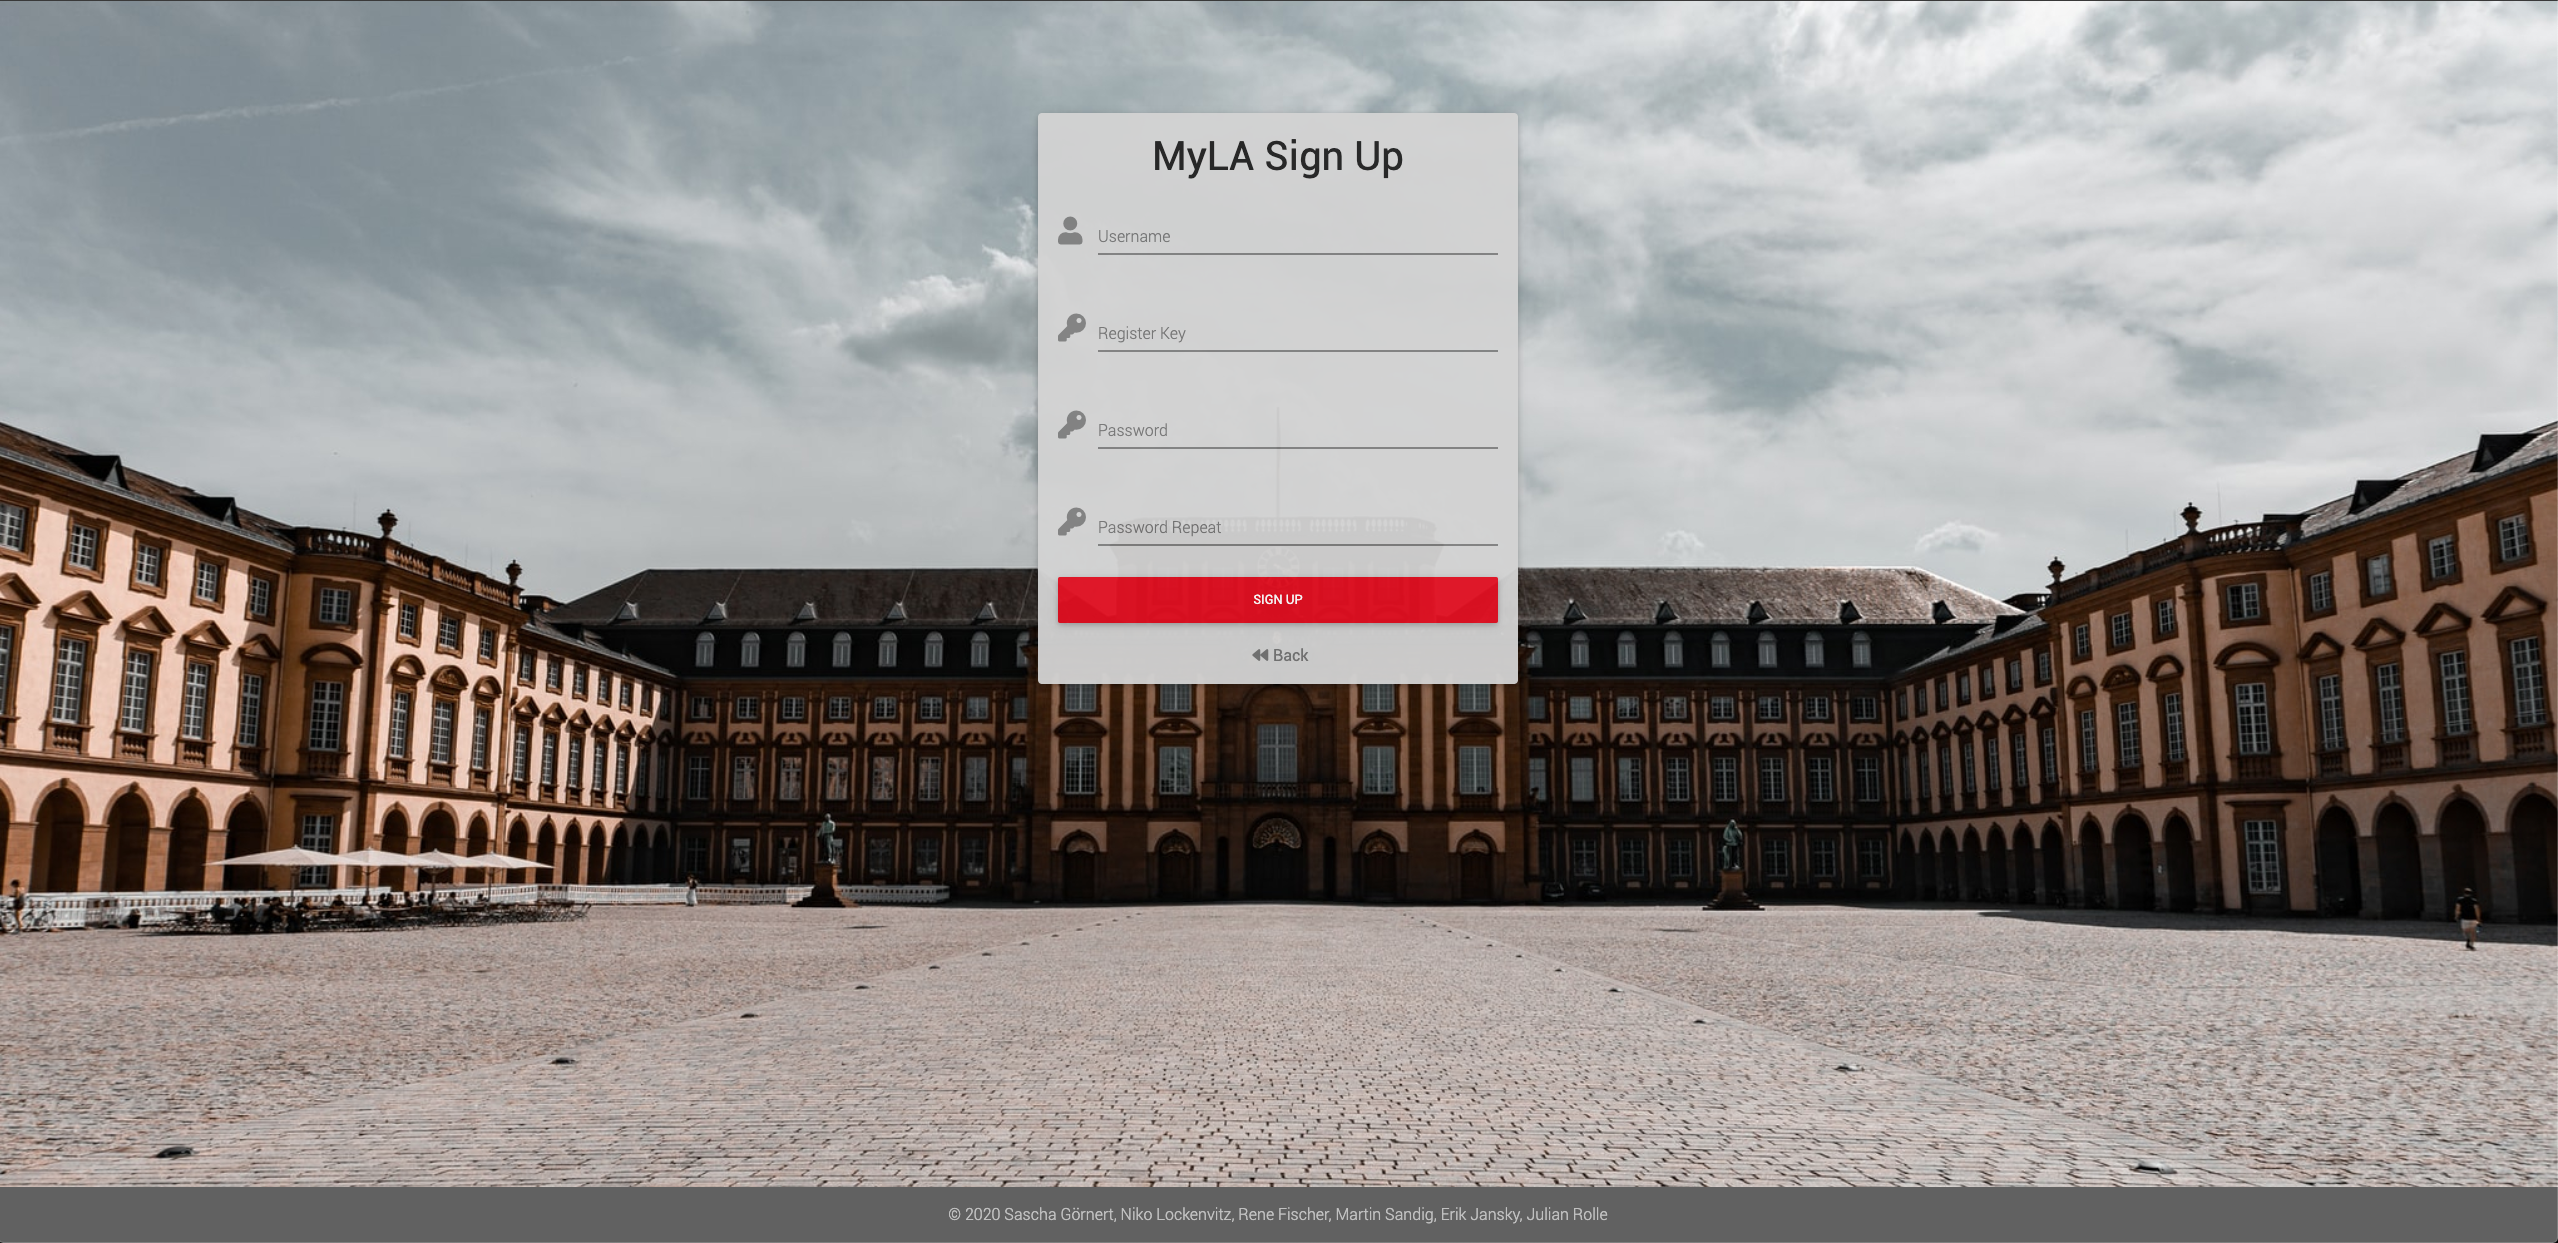
\includegraphics[width=0.95\textwidth, keepaspectratio]{img/client/Signup.png}
	\captionsetup{justification=centering, format=plain}
	\caption[\acl{UI}: Registrierung]{\acl{UI}: Registrierung \\ \quelleScreenshot}
	\label{fig:SignupImplement}
\end{figure}
